\section{DNS}
\subsection{DNS refresher}

The Domain Name System (DNS) is a distributed naming system that allows clients to translate domain names into IP addresses. For example, an \texttt{A} record maps a domain name to an IPv4 address, while an \texttt{AAAA} record maps it to an IPv6 address. DNS can also store many other types of information, such as mail servers (\texttt{MX}) or aliases (\texttt{CNAME}).

Domain names are organized hierarchically as a tree. For example, the domain name \texttt{git.louvainlinux.org.} is composed of the following levels:

\begin{itemize}
    \item The root domain \texttt{.}
    \item The top-level domain \texttt{org}
    \item The domain \texttt{louvainlinux.org}
    \item The host or subdomain \texttt{git}
\end{itemize}

To resolve a domain name, a recursive DNS resolver queries the DNS hierarchy step by step. The root servers return the name servers responsible for \texttt{.org}, the \texttt{.org} servers return the name servers responsible for \texttt{louvainlinux.org}, and finally the authoritative server for \texttt{louvainlinux.org} (in our case OVH's servers) returns the requested record for \texttt{git.louvainlinux.org}, our public IP.


The servers responsible for a DNS zone are called \texttt{authoritative name servers}.


\subsection{Cache poisoning}
Resolvers may often have to resolve the same domain names (\texttt{google.com}, \texttt{instagram.com},...) and in order to be more efficient, the use caching. When a request having already been answered is received, it doesn't resolve it again but looks in its table. Records have a \texttt{TTL} : time to live.

Caching is also done inside our computer for the same reasons.

Caches can be exploited in \texttt{cache poisoning attacks} where an attacker takes advantage of the fact that the cache might be less protected than the data source. Both presented attacks are used in order to redirect the traffic for a targetted website. This could be useful for fishing, steal information or do Denial-of-Service attack by denying the access to the targetted website.

\subsubsection{First variant}

Previously, authoritative DNS servers were allowed to include additional DNS records in their responses, even when those records were not requested. This could be exploited for DNS cache poisoning.

For example, an attacker controlling the authoritative server for \texttt{evil.com}
could respond to a query for \texttt{www.evil.com} with the correct answer, but also
include a forged record claiming that \texttt{www.bank.com} resolves to the attacker's
IP address. If the recursive resolver cached this additional record, a later request
for \texttt{www.bank.com} could be answered using the poisoned cache, redirecting
users to a malicious website instead of the legitimate one.

Modern resolvers prevent this by doing a \textit{Bailiwick Check} : accept additional records only if they contain
information about the same domain as in the request.
\begin{figure}
    \centering
    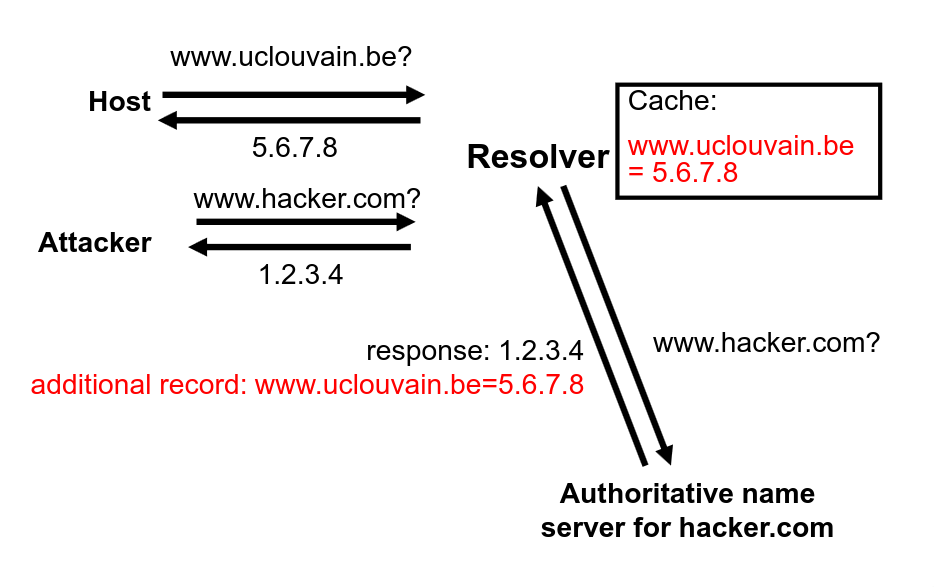
\includegraphics[width=0.7\linewidth]{Figures/DNS_1.png}
    \caption{DNS Cache Poisoning 1}
\end{figure}
\subsubsection{Second variant}
In the second  version an attacker sends a fake response to the DNS resolver spoofing the IP address of the Authoritative Name Server supposed to answer the actual query. This is possible because DNS is built over UDP which makes the resolver un-aware of a possible connection state with the Authoritative NS.
\begin{figure}
    \centering
    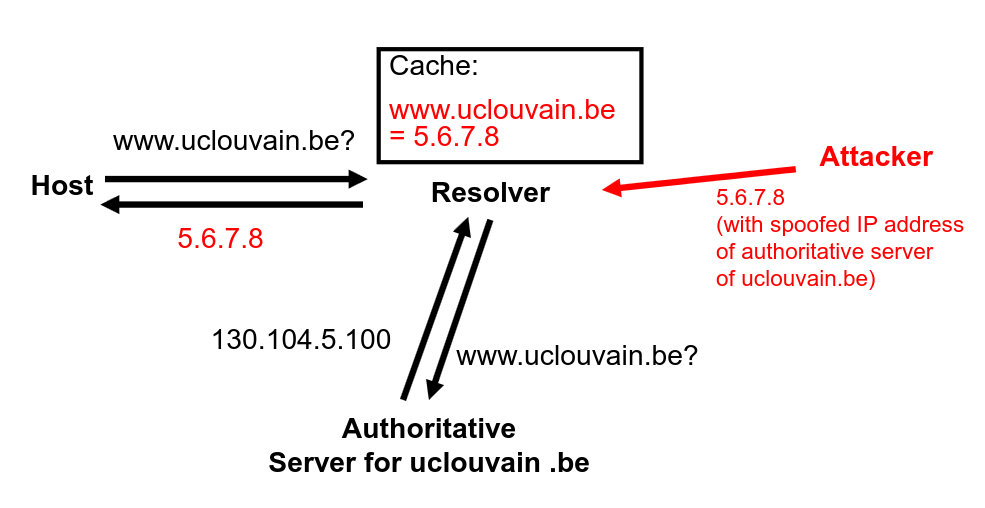
\includegraphics[width=0.7\linewidth]{Figures/DNS_2.png}
    \caption{DNS Cache Poisoning 2}
\end{figure}


In reality this attack is a little more complicated to execute beacause of two verifications : 
\begin{itemize}
    \item A \texttt{DNS query ID} that is sent to the DNS server which answer must contain this ID,
    \item The response must be sent to the same UDP port from which the query originated.
\end{itemize}

So an attacker would have to guess both numbers for the resolver to accept the spoofed packet which is unlily to happen. Though old DNS servers are still vulnerable as consistent ports and predictable \texttt{DNS query ID} were used.

\subsubsection{ARP Cache Poisoning (or ARP Spoofing)}
Reminder that \texttt{ARP} (\textbf{Address Resolution Protocol}) is used to resolve the MAC address corresponding to an IPv4 address (\textbf{Neighbor Discovery Protocol} is used for IPv6). Each host maintains its own ARP cache and broadcasts ARP requests when it needs to determine the MAC address associated with an IP address on the local network.

Since ARP does not authenticate replies and hosts typically accept unsolicited ARP responses, an attacker present on the same local network can perform an \textit{ARP poisoning} attack. By sending forged ARP replies that associate a victim's IP address (e.g., the default gateway) with the attacker's MAC address, the attacker can redirect traffic through their machine and potentially perform a man-in-the-middle attack.

\subsubsection{Web Cache Poisoning}
Web cache poisoning occurs when an attacker causes a cache to store a malicious HTTP response that will later be served to other users requesting the same resource. An attacker relies on a page that includes user-controlled input. By injecting malicious content, they can cause the server to generate a poisoned response. If the cache does not differentiate between requests containing the malicious input and normal requests, the poisoned response may be cached and subsequently served to legitimate users.


